\setcounter{chapter}{-1}
\chapter{Introduction and Context}
\label{chap.intro}

In this thesis, we study the homotopy of configuration spaces of manifolds using ideas coming from the theory of operads.
These configuration spaces consist of collections of pairwise distinct points in a given manifold.
We address the problems of their homotopy invariance and the definition of rational models for them.
We adapt constructions of Kontsevich~\cite{Kontsevich1999}, who proved the formality of (compactified) configuration spaces of Euclidean spaces as an operad.

The notion of an operad was initially introduced for the study of iterated loop spaces in homotopy theory~\cite{May1972,BoardmanVogt1973}.
The theory of operads has been considerably renewed since the mid-nineties, when, after insights of Kontsevich~\cite{Kontsevich1993a}, Ginzburg and Kapranov~\cite{GinzburgKapranov1994} proved in a seminal work that some duality phenomena in algebra could be interpreted in terms of operads.
Since then, a number of new applications of operads have been discovered in several fields of mathematics.

In this introduction, we first explain what operads are in Section~\ref{intro.sec.operads}.
Then we describe two important families of operads, the little disks operads (Section~\ref{intro.sec.little-disks-operads}) and the Swiss-Cheese operads (Section~\ref{sec.swiss-cheese-operads}).
In Section~\ref{intro.sec.configuration-spaces}, we turn to configuration spaces of manifolds.
Section~\ref{intro.sec.closed-manifolds} is devoted to closed manifolds, whereas Section~\ref{sec.comp-manif-with} is about compact manifolds with boundary.

\section{Operads}
\label{intro.sec.operads}

Roughly speaking, an operad is an object that governs a category of algebras.
The central idea can be understood by analogy with the theory of group representations.
In this analogy, the operad corresponds to the group, and the algebras over the operad correspond to the representations of the group.

If a group is given with a presentation by generators and relations, then the associated category of representations can also be defined in terms of the actions of the generators, which have to satisfy the relations.
In our analogy, a category of algebras is defined in terms of generating operations and relations.
For example, the structure of an associative algebra is defined in terms of a product as a generating operation together with associativity as a relation.
The structure of a commutative algebra is defined similarly, with the condition that the product is symmetric, Lie algebras are defined in terms of an antisymmetric Lie bracket and the Jacobi relation, and so on.
Each of these definitions can be interpreted as the definition of an operad by generators and relations which governs the given category of algebras.

It is interesting to study the operad itself, independently of any presentation by generators and relations, just like we study groups.
This new perspective enables us to consider morphisms, sub-operads, quotients, extensions\dots{}
Knowledge about an operad then translates into knowledge about algebras over that operad.

Let us explain more precisely what operads are.

\begin{wrapfigure}{l}{0.3\textwidth}
  \centering
  \vspace{-5mm}
  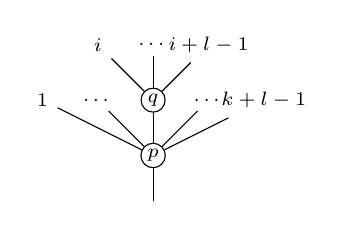
\begin{tikzpicture}[font=\scriptsize, grow'=up, level 1/.style={sibling distance=2em, level distance=2em}]
    \node{}
    child {
      node[draw, circle, inner sep = 1 pt] {$p$}
      child {node {$1$}}
      child {node {\dots}}
      child {
        node[draw, circle, inner sep = 1pt] {$q$}
        child {node {$i$}}
        child {node {\dots}}
        child {node {$i+l-1$}}
      }
      child {node {\dots}}
      child {node{$k+l-1$}}
    }
    ;
  \end{tikzpicture}
  \vspace{-5mm}
\end{wrapfigure}


The algebraic structures governed by operads are those that can be described in terms of operations with a finite number of inputs and exactly one output.
An operad\footnote{To be precise, by an ``operad'' we mean a symmetric, one-colored operad. There exists other variants: non-symetric operads, cyclic operads, colored operads, etc.} $\PP$ is a collection $\PP = \{ \PP(k) \}_{k \ge 0}$ of abstract ``operations''.
An element of $\PP(k)$ can be viewed as a operation with $k$ inputs (``of arity $k$'') and one output.
There is an action of the symmetric group $\Sigma_{k}$ on $\PP(k)$ which models the permutations of the input of an operation.
There are insertion morphisms:
\[ \circ_{i} : \PP(k) \otimes \PP(l) \to \PP(k+l-1), \quad 1 \leq i \leq k, \]
which model composition of operations, similarly to how multiplication in a group $G$ corresponds to composition of operations on representations.
Finally, there is an identity $\id \in \PP(1)$ which is a neutral element for composition.

To illustrate this definition, one can look at the prototypical example, the \emph{endomorphism operad}.
Given some object $X$ in a symmetric monoidal category, the endomorphism operad $\End_{X}$ is defined by $\End_{X}(n) \coloneqq \Hom(X^{\otimes n}, X)$.
The symmetric group action acts by permuting inputs:
\[ (f \cdot \sigma)(x_{1}, \dots, x_{k}) = f(x_{\sigma(1)}, \dots, x_{\sigma(k)}), \]
and the insertion operation is given by composition of morphisms:
\[ (f \circ_{i} g)(x_{1}, \dots, x_{k+l-1}) = f(x_{1}, \dots, x_{i-1}, g(x_{i}, \dots, x_{i+l-1}), x_{i+l}, \dots, x_{k+l-1}). \]
Finally, the identity $\id \in \End_{X}(1)$ is simply the identity of $X$.
An algebra $X$ over an operad $\PP$ is by definition a morphism of operads $\PP \to \End_{X}$, just like a group representation is a morphism $G \to \operatorname{End}(V)$.
As another example, an operad with only operations of arity $1$ is the same thing as a monoid, and an algebra over such an operad is the same thing as a representation of the corresponding monoid.
We refer to the books~\cite{LodayVallette2012,Fresse2017} for a more extensive treatment of operads.

\subsection{Little disks operads}
\label{intro.sec.little-disks-operads}

There exists a certain family of topological operads of particular interest, the little $n$-disks operads $\DD_{n}$ (or equivalently, the little $n$-cubes operads).
These are precisely the operads which appeared in the original study of iterated loop spaces.

\begin{wrapfigure}{R}{0.2\textwidth}
  \centering
  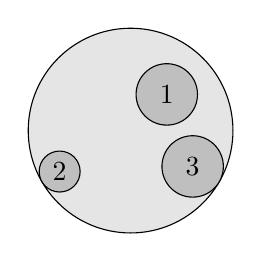
\begin{tikzpicture}[scale=1.3]
    \coordinate (a) at (45:0.5);
    \coordinate (b) at (210:0.8);
    \coordinate (c) at (-30:0.7);
    \filldraw [fill = gray!20] (0,0) circle (1);
    \filldraw [fill = gray!50] (a) circle (0.3) node {1};
    \filldraw [fill = gray!50] (b) circle (0.2) node {2};
    \filldraw [fill = gray!50] (c) circle (0.3) node {3};
  \end{tikzpicture}
\end{wrapfigure}


An element of $\DD_{n}(k)$ is an ordered configuration of $k$ little $n$-disks with disjoint interiors in the unit disk $D^{n}$.
Each disk of the configuration represents an embedding of $D^{n}$ into itself, obtained by the composition of a translation and a positive homothety.
The set $\DD_{n}(k)$ is endowed with the compact-open topology of embeddings.
The symmetric group action renumbers the disks in a configuration, and insertion is given by composition of embeddings.

\begin{figure}[htbp]
  \centering
  \begin{tikzpicture}[scale=2]
  \coordinate (a) at (45:0.5);
  \coordinate (b) at (210:0.5);
  \coordinate (c) at (-30:0.8);
  \coordinate (d) at (80:0.5);
  \coordinate (e) at (0:0.7);

  \filldraw [fill = gray!20] (0,0) circle (1);
  \filldraw [fill = gray!50] (a) circle (0.4) node {1};
  \filldraw [fill = gray!50] (b) circle (0.5) node {2};
  \filldraw [fill = gray!50] (c) circle (0.2) node {3};

  \draw (1.3, 0) node {$\circ_{2}$};

  \coordinate (x1) at (2.5,0);
  \filldraw [fill = gray!20] (x1) circle (1);
  \filldraw [fill = gray!60!blue] ($(d) + (x1)$) circle (0.4) node {1};
  \filldraw [fill = gray!60!blue] ($(e) + (x1)$) circle (0.2) node {2};

  \draw (3.75, 0) node {$=$};

  \coordinate (x2) at (5,0);
  \filldraw [fill = gray!20] (x2) circle (1);
  \filldraw [fill = gray!50] ($(a) + (x2)$) circle (0.4) node {1};
  \draw [dashed] ($(b) + (x2)$) circle (0.5);
  \filldraw [fill = gray!50] ($(c) + (x2)$) circle (0.2) node {4};

  \coordinate (x3) at ($(x2) + (-0.433, -0.25)$); % cos(210)/2, sin(210)/2
  \filldraw [fill = gray!60!blue] ($1/2*(d) + (x3)$) circle (0.2) node {2};
  \filldraw [fill = gray!60!blue] ($1/2*(e) + (x3)$) circle (0.1) node {3};
\end{tikzpicture}

  \caption{Composition of embeddings}
  \label{intro.fig.compos-embed}
\end{figure}

Almost by definition, an $n$-fold loop space $\Omega^{n} X$ is a $\DD_{n}$-algebra.
The ``recognition principle''~\cite{May1972,BoardmanVogt1973} asserts that the converse is true: under technical conditions, a (grouplike) $\DD_{n}$-algebra is weakly homotopy equivalent to an $n$-fold loop space.

Since this first homotopy-theoretical application, the little disks operads have proved to be useful in a number of settings.
Let us mention the Deligne conjecture~\cite{KontsevichSoibelman2000,McClureSmith2002}, which asserts that the Hochschild cochains $C^{*}(A;A)$ of an associative algebra are equipped with an action of $\DD_{2}$; the formality theorem for Hochschild cochains and its application to deformation quantization of Poisson manifolds~\cite{Kontsevich1999,Tamarkin1998,Kontsevich2003}; Goodwillie--Weiss calculus and the computation of embedding spaces and long knots~\cite{Sinha2006,LambrechtsTurchinVolic2010,AroneTurchin2014,DwyerHess2012,BoavidaWeiss2013}, as well as the ``covariant version'' of embedding calculus that is factorization homology~\cite{BeilinsonDrinfeld2004,Lurie2009,Lurie2016,AyalaFrancis2015,CostelloGwilliam2017}.

A fundamental result about the little disks operads is that they are \emph{formal} over $\Q$~\cite{Kontsevich1999,Tamarkin2003,LambrechtsVolic2014,FresseWillwacher2015}: the operad of chains $C_{*}(\DD_{n}; \Q)$ is quasi-isomorphic to its homology $\en \coloneqq H_{*}(\DD_{n}; \Q)$.
Thus it suffices to study the operads $\en$, which have a simple combinatorial description: $\en[1] = \Ass$ governs associative algebras, and for $n \ge 2$, $\en$ governs $(n-1)$-Poisson algebras~\cite{Cohen1976}.
When $n = 2$, the formality of $\DD_{2}$ depends on the choice of a Drinfeld associator, something which gives a universal way to build a braided monoidal category out of some Lie-algebraic data (see e.g.~\cite[Chapter~I.10]{Fresse2017} for details).

\subsection{The Swiss-Cheese operads}
\label{sec.swiss-cheese-operads}

Colored operads (a.k.a.\ multicategories), a generalization of operads, are used to describe algebraic structures shaped on multiple objects.
In this setting, the inputs and the output of an operation are all labeled by ``colors'', and composition is only defined if the colors match.
In the definition of an algebra over such a colored operad, each color corresponds to a given object.

\begin{wrapfigure}{l}{0.3\textwidth}
  \centering
  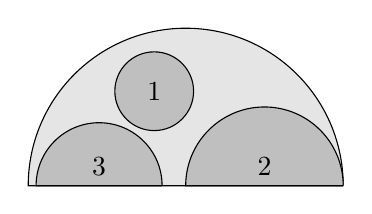
\begin{tikzpicture}
    \filldraw [fill = gray!20] (2,0) arc (0:180:2) -- (2,0);
    \filldraw [fill = gray!50] (2,0) arc (0:180:1) -- node[above] {$2$} (2,0);
    \filldraw [fill = gray!50] (-0.3,0) arc (0:180:0.8) -- node[above] {$3$} (-0.3,0);
    \filldraw [fill = gray!50] (-0.4,1.2) circle (0.5) node {$1$};
  \end{tikzpicture}
\end{wrapfigure}


The Swiss-Cheese operad $\SC = \SC_{2}$~\cite{Voronov1999} is a $2$-colored operad which governs the action of a $\DD_{2}$-algebra on a $\DD_{1}$-algebra by a central morphism.
An operation in $\SC$ is given by the embedding of disks and upper half-disks in the unit upper half-disk.
It is related to the OCHAs of Kajiura--Stasheff~\cite{KajiuraStasheff2006a,Hoefel2009} and there is a Swiss-Cheese version of the Deligne conjecture~\cite{DolgushevTamarkinTsygan2011}.
Higher dimensional variants $\SC_{n}$ govern the action of a $\DD_{n}$-algebra on a $\DD_{n-1}$-algebra.

Unlike the little disks operads, the Swiss-Cheese operads are not formal~\cite{Livernet2015} and one cannot recover $\SC_{n}$ from $\Sc_{n} = H_{*}(\SC_{n})$ over $\Q$.
Our first goal in this thesis was to find a model for the Swiss-Cheese operad $\SC_{2}$ that fixes this lack of formality.
The homology $\Sc_{2}$ splits as a ``Voronov product'' $\en[2] \otimes \en[1]$ and governs the action of a Gerstenhaber algebra on an associative algebra via a central map.
Theorem~\ref{sw.thm.A} describes a model in groupoids for $\SC_{2}$ which governs the action of a braided monoidal category on a monoidal category via a central monoidal functor.
Theorem~\ref{sw.thm.B} describes a model over $\Q$ for $\SC_{2}$, which uses a Drinfeld associator to construct a kind of ``twisted'' Voronov product between a rational model for $\en[2]$ (built out of chord diagrams) and a model for $\en[1]$.

\section{Configuration spaces}
\label{intro.sec.configuration-spaces}

\subsection{Closed manifolds}
\label{intro.sec.closed-manifolds}

Let $M$ be an $n$-dimensional manifold; its $k$th configuration space is:
\[ \Conf_{k}(M) = \{ x \in M^{k} \mid \forall 1 \leq i < j \leq k, x_{i} \neq x_{j} \}. \]

This construction is obviously not homotopy invariant for open manifolds when $k \geq 2$, as for example $\Conf_{2}(\R^{n}) \simeq S^{n-1}$ for $n \in \mathbb{N}$.
Even if we restrict our attention to closed manifolds, $\Conf_{k}(-)$ is still not a homotopy invariant~\cite{LongoniSalvatore2005}.
The counterexample (lens spaces) is not simply connected, and the homotopy invariance for simply connected closed manifolds remains an open question.

Some results are known.
The homotopy type of $\Omega \Conf_{k}(M)$ only depends on the homotopy type of $(M, \partial M)$ for connected compact manifolds~\cite{Levitt1995}.
Configuration spaces are also known to be a \emph{stable} homotopy invariant~\cite{AouinaKlein2004} of closed manifolds.
If $M$ is a smooth projective complex manifold, then the rational homotopy type of $\Conf_{k}(M)$ only depends on the one of $M$~\cite{Kriz1994}.
The same result holds for $k = 2$ when $M$ is a closed manifold and either $2$-connected~\cite{LambrechtsStanley2004} or simply connected and even dimensional~\cite{CordovaBulens2015}.

We prove, as a corollary of the main result of Chapter~\ref{chap.2} (Theorem~\ref{cnf.thm.A}), that the real homotopy type of $\Conf_{k}(M)$ only depends on the real homotopy type of $M$ when the manifold is closed, smooth, simply connected and of dimension at least $4$.

When working over $\Q$ (or $\R$) with simply connected manifolds, we can use Sullivan's~\cite{Sullivan1977} theory of rational models to study topological spaces up to rational equivalence.
Closed, simply connected manifolds are known to have models satisfying a kind of chain-level Poincaré duality~\cite{LambrechtsStanley2008}.
Out of a Poincaré duality model of $M$, we give an explicit real model for $\Conf_{k}(M)$.
This model had been conjectured by Lambrechts--Stanley~\cite{LambrechtsStanley2008a} in the general case, and had previously been studied in some special cases~\cite{CohenTaylor1978,BenderskyGitler1991,Kriz1994,Totaro1996,FelixThomas2004,LambrechtsStanley2004,CordovaBulens2015}.

Our proof relies on Kontsevich's proof of the formality of the little disks operads.
The configuration spaces $\Conf_{k}(\R^{n})$ admit compactifications $\FM_{n}(k)$ due to Fulton--MacPherson~\cite{FultonMacPherson1994} (and Axelrod--Singer~\cite{AxelrodSinger1994} in the real case).
An element of $\FM_{n}(k)$ can roughly be seen as a configuration of $k$ points in $\R^{n}$, where the points are allowed to become ``infinitesimally close''.
One can insert such an infinitesimal configuration into another, and the spaces $\FM_{n}(-)$ assemble into an operad weakly equivalent to the little disks operads.
Kontsevich's proof uses piecewise semi-algebraic (PA) forms and integrals along the fiber to build an explicit equivalence between $C_{*}(\FM_{n})$ and $\en$.

Similarly, if $M$ is a closed manifold, then $\Conf_{k}(M)$ can be compactified into $\FM_{M}(k)$.
If $M$ happens to be framed, then the spaces $\FM_{M}(-)$ assemble to form a right module over the operad $\FM_{n}$.
This extra structure is what allows us to prove Theorem~\ref{cnf.thm.A}.
When $M$ is framed, we then obtain that the action of the little disks operad on the configuration spaces is compatible with our model.
We are able, using this additional result and a comparison statement between the Cohen--Taylor spectral sequence~\cite{CohenTaylor1978} and the Bendersky--Gitler spectral sequence~\cite{BenderskyGitler1991} established by Félix--Thomas~\cite{FelixThomas2004}, to recover a theorem of Knudsen~\cite{Knudsen2016} about the factorization homology of a framed manifold with coefficients in the higher enveloping algebra of a Lie algebra.

\subsection{Compact manifolds with boundary}
\label{sec.comp-manif-with}

In the last chapter, we study configuration spaces of compact manifolds with boundary.
As for closed manifolds, homotopy invariance of configuration spaces of compact manifolds with boundary is an open question.
It is known that if the manifold and its boundary are both $2$-connected, then the rational homotopy type of $\Conf_{2}(M)$ only depends on the rational homotopy type of the pair $(M, \partial M)$~\cite{CordovaBulensLambrechtsStanley2015a}.

The manifolds we consider are those which admit a ``Poincaré--Lefschetz duality model''
These are a generalization of surjective pretty models as defined in~\cite{CordovaBulensLambrechtsStanley2015}.
Briefly, if $N$ is a closed manifold and $K \subset N$ is a sub-polyhedron, to obtain a model for $M = N - K$ one takes a Poincaré duality model for $N$ and then ``kills'' (using a mapping cone) the cohomology classes coming from $K$.
We can apply these ideas to manifolds with boundary which are obtained by removing an open neighborhood of a sub-polyhedron from a closed manifold.
Manifolds admitting a surjective pretty model include closed manifolds, $2$-connected manifolds with $2$-connected boundary satisfying an algebraic retraction property, disk bundles of even rank of simply connected closed manifolds, and spaces obtained by removing a high-codimensional sub-polyhedron from a $2$-connected manifold~\cite{CordovaBulensLambrechtsStanley2015,CordovaBulensLambrechtsStanley2015a} (see Theorem~\ref{cnfbnd.thm.pretty-model} for details).
More generally, if $M$ is simply connected with simply connected boundary, we can prove that it admits a Poincaré--Lefschetz duality model as soon as $n \geq 7$, and we recover the same results.

We first use a kind of chain-level Poincaré--Lefschetz duality and cubical diagrams to compute the Betti numbers of $\Conf_{k}(M)$, as was done for closed manifolds in~\cite{LambrechtsStanley2008a}.
We then reuse the methods of Chapter~\ref{chap.2} to provide an explicit real model for $\Conf_{k}(M)$.
One must adapt the Fulton--MacPherson compactifications to deal with the boundary of $M$, and we obtain as Theorem~\ref{cnfbnd.thm.A} that the model conjectured in~\cite{CordovaBulensLambrechtsStanley2015a} is a real model for $\Conf_{k}(M)$.
This model only depends on a model of $M$, therefore, as a corollary, we obtain the real homotopy invariance of $\Conf_{k}(-)$ for smooth simply connected manifolds with simply connected boundary of dimension $\geq 5$ (either admitting a pretty model or of dimension $\geq 7$).

The compactified configuration spaces on a framed manifold with boundary inherit an action of an operad $\SFM_{n}$, weakly equivalent to the Swiss-Cheese operad $\SC_{n}$.
In Theorem~\ref{cnfbnd.thm.B}, we describe a model for the resulting module over $\SFM_{n}$, using a graphical model of $\SC_{n}$ found by Willwacher~\cite{Willwacher2015a}.
